\section{Generating the control flow graph}

The body of the \code{while} statement previously generated contains a \code{switch} statement, whose body itself
contains \code{case}s for each \textit{basic block} in the original body of the method, as defined below.

Because the Java programming language does not provide a \code{goto} statement, there is no direct a way of jumping at
a later point in code (useful when returning from a recursive call to execute the statements after the call). But this
problem can be solved if the code is broken into \textit{basic blocks}, by generating the control flow graph of the
method body. Each basic block corresponds to a \code{case} inside the \code{switch} statement from above. Jumping
between different blocks is possible by using the \code{block} field of the \code{frame} object.

The structure of the CFG (Control Flow Graph) \abbrev{CFG}{Control Flow Graph} presented here is inspired from LLVM
IR (Intermidiate Representation)\abbrev{IR}{Intermidiate Representation}\footnote{\url{https://llvm.org/docs/LangRef.html}}.

In this context, a \code{Block} is defined as a list of non-terminal \code{NormalStatement}s terminated by a
\code{TerminatorStatement}. This definition is inspired from the definition of a \textit{basic block} as presented in
\textit{Chapter 8.4} of \cite{aho}.

A \code{NormalStatement} is a wrapper over a \code{PsiStatement}.

A \code{TerminatorStatement} is either a \code{ReturnStatement}, a \code{ConditionalJumpStatement}, an
\code{UnconditionalJumpStatement} or a \code{SwitchStatement}.

A \code{ReturnStatement} is a wrapper over a \code{PsiReturnStatement}.

A \code{ConditionalJumpStatement} jumps from the containing \code{Block} to one of two \code{Block}s, based on the
value of a \code{PsiExpression}.

An \code{UnconditionalJumpStatement} jumps from the containing \code{Block} to another \code{Block}.

A \code{SwitchStatement} corresponds to a \code{PsiSwitchStatement}. It jumps to one of multiple blocks corresponding to
the blocks in the body of the original \code{PsiSwitchStatement}, based on its associated \code{PsiExpression}.

The list of \code{Block}s for the method body is generated by a \code{JavaRecursiveElementVisitor}, which performs
different operations for each type of \code{PsiElement} encountered. Each \code{Block} has an \code{id} field which
represents the label of its corresponding \code{case}.

The visitor initializes a \code{myCurrentBlock} field before visiting the actual body of the method. This is the entry
block of the function. The visitor also keeps two private mappings\\
(\code{myBreakTargets} and \code{myContinueTargets})
from potential \code{break} and \code{continue} target statements (\code{for}, \code{while}, \code{do-while} loops and
\code{switch} statements) to the basic blocks to which control flow jumps after executing the corresponding
\code{break} or \code{continue} statement. The following subsections present how the visitor processes each type of
relevant \code{PsiElement} encountered.

\subsection{Visiting a \code{PsiCodeBlock}}

The body of a method is represented as a \code{PsiCodeBlock}. The visitor processes each\\
\code{PsiStatement} in the \code{PsiCodeBlock}.

In this context, processing means that if the \code{PsiStatement} contains recursive calls or is an instance of
\code{PsiReturnStatement}, \code{PsiBreakStatement} or \code{PsiContinueStatement},
it accepts the visitor for further processing.

Otherwise, a \code{BreakContinueReplacerVisitor} visits the \code{PsiStatement} in order to replace the \code{break} and
\code{continue} statements with inlined \code{UnconditionalJumpStatement}s to the target \code{block}s of these
statements. The only statements affected are those whose exited or continued statement has been previously visited by
the CFG generator. The target \code{block}s of these statements also get their \code{doNotInline} flag set to \code{true},
so as not to be inlined by later passes. Here, an inlined \code{UnconditionalJumpStatement} means an assignment to the
\code{block} field of the \code{frame} object with the \code{id} of the target \code{block}, followed by a \code{break}
statement. After the replacer visitor processing finishes, a \code{NormalStatement} wrapper over the
\code{PsiStatement} is added to the \code{myCurrentBlock}.

An important last step after processing all the \code{PsiStatement}s in the \code{PsiCodeBlock} of the method is adding
an explicit \code{ReturnStatement} to the \code{myCurrentBlock}, if the return type of the method is \code{void} and the
body does not already contain an explicit \code{return} statement. This is almost always the case because these methods
do not specify a final \code{return} statement, since it is redundant.

\subsection{Visiting a \code{PsiBlockStatement}}
Since the \code{PsiBlockStatement} is merely a wrapper over a \code{PsiCodeBlock}, visiting it translates to processing
the statements of its contained \code{PsiCodeBlock}, just as already specified above.

\subsection{Visiting a \code{PsiReturnStatement}}

A \code{ReturnStatement} wrapper over the \code{PsiReturnStatement} is added to the\\
\code{myCurrentBlock}.

\subsection{Visiting a \code{PsiBreakStatement}}

The \code{exitedStatement} corresponding to the \code{break} statement is computed. If the\\
\code{exitedStatement} is not contained in the \code{myBreakTargets} map, a \code{NormalStatement} wrapper over
the \code{PsiBreakStatement} is added to the \code{myCurrentBlock}. Otherwise, an \code{UnconditionalJumpStatement} to
the target \code{block} is added to the \code{myCurrentBlock}.

\subsection{Visiting a \code{PsiContinueStatement}}

The \code{continuedStatement} corresponding to the \code{continue} statement is computed. If the \code{continuedStatement}
is not contained in the \code{myContinueTargets} map, a \code{NormalStatement} wrapper over the \code{PsiContinueStatement}
is added to the \code{myCurrentBlock}. Otherwise, an \code{UnconditionalJumpStatement} to the target \code{block} is added
to the \code{myCurrentBlock}.

\subsection{Visiting a \code{PsiMethodCallExpression}}

Given the previous passes and the processing of \code{PsiStatement}s presented above, the visitor actually visits only
recursive calls. These calls appear only as right-hand sides of\\
\code{PsiAssignmentExpression}s or as initializers of \code{PsiVariable}s in\\
\code{PsiDeclarationStatement}s (generated by the \textit{Extracting recursive calls to statements} pass).

The recursive call is transformed in a \code{push} call to the \code{stack}, where the new \code{frame} object is
initialized using the \code{PsiExpression}s provided as arguments to the recursive call. A new \code{Block} is generated
and it is marked so as not to be inlined by a later pass. Then an \code{UnconditionalJumpStatement} which jumps to the
new block is added to the\\
\code{myCurrentBlock}. After this, the \code{myCurrentBlock} is changed to the new block. The
\code{PsiStatement} in which the recursive call appears is added to the new \code{myCurrentBlock}, but having the
recursive call replaced with a \code{PsiExpression} referring to the \code{ret} variable.

\subsection{Visiting an \code{PsiIfStatement}}

Two new blocks are generated: the \code{thenBlock} and the \code{mergeBlock}. An optional third block (the
\code{elseBlock}) gets generated if the \code{if} statement has an \code{else} branch. A\\
\code{ConditionalJumpStatement} is added to the \code{myCurrentBlock}. It jumps to either the \code{thenBlock} or the
\code{elseBlock}. If there is no \code{elseBlock}, it jumps to the \code{mergeBlock} instead.

The \code{myCurrentBlock} is set to the \code{thenBlock} and the \code{then} branch accepts the visitor. After this,
an \code{UnconditionalJumpStatement} to the \code{mergeBlock} is added to the \code{myCurrentBlock}, which may be other
than the \code{thenBlock}, because of the visitor possibly changing it when visiting the \code{then} branch.

If there is an \code{else} branch, it is treated similarly to the \code{then} branch. Finally, the\\
\code{myCurrentBlock} is set to the \code{mergeBlock}.

The description above is depicted in \labelindexref{Figure}{img:if-statement}. The grey boxes represent basic blocks
which are optional and the dotted lines represent arbitrary subgraphs.

\begin{figure}[htb]
    \centering
    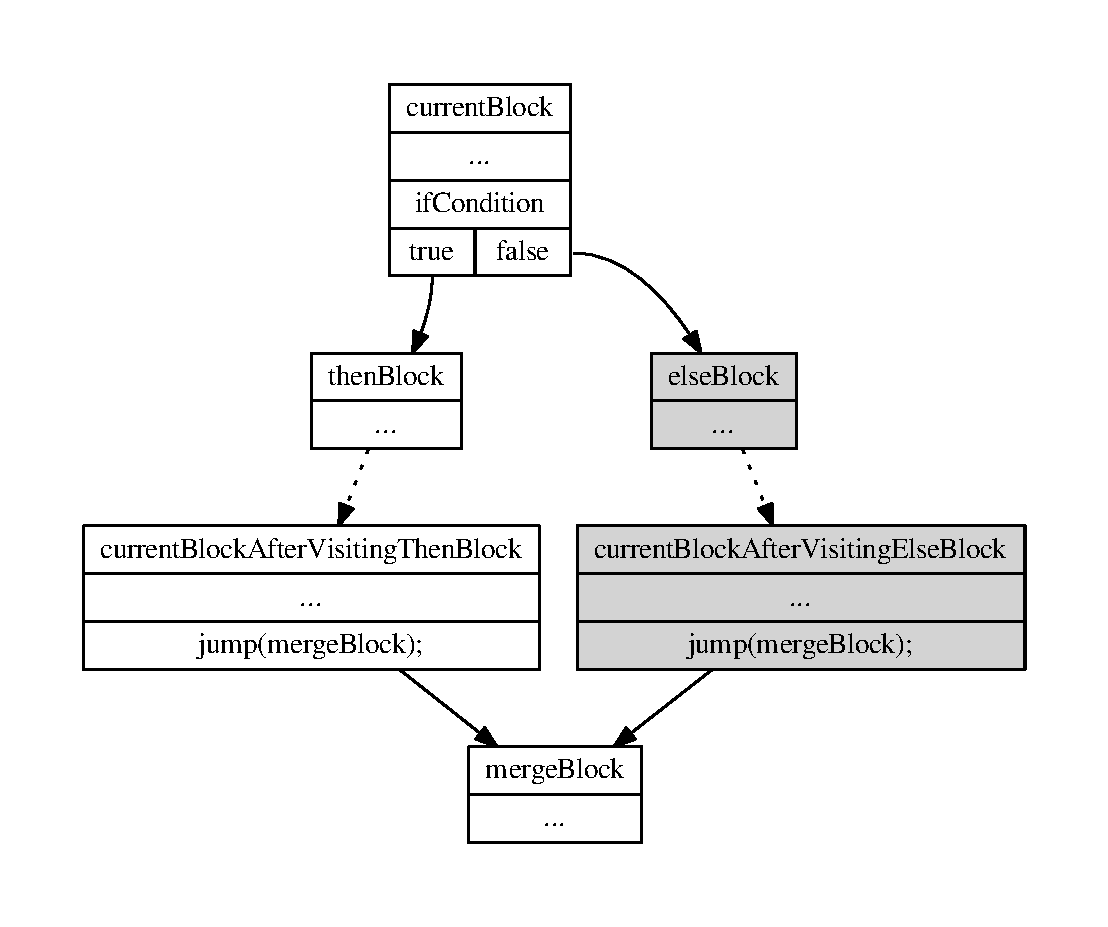
\includegraphics[width=.5\textwidth]{src/graph/if.pdf}
    \caption{If statement CFG\label{img:if-statement}}
\end{figure}

\subsection{Visiting loop statements}

There are four possible types of loop statements in a Java PSI tree: \code{PsiWhileStatement},
\code{PsiDoWhileStatement}, \code{PsiForeachStatement} and \code{PsiForStatement}. The\\
\code{PsiForeachStatement}s have been replaced with equivalent \code{PsiForStatement}s in the \textit{Replacing
\code{foreach} loops with \code{for} loops} pass. The other three types of loop statements are similar, with
\code{PsiWhileStatement} and \code{PsiDoWhileStatement} being special cases of \code{PsiForStatement}.

In the case of a \code{PsiForStatement}, if it has any initialization, the corresponding\\
\code{PsiStatement}s are added to the \code{myCurrentBlock}. There are three cases here, based on how Intellij IDEA
parses the initialization part of a \code{for} statement. If the initialization is an instance of
\code{PsiEmptyStatement}, there is no actual statement to add. If the initialization is an instance of
\code{PsiExpressionStatement}, this statement is added to the \code{myCurrentBlock}. Finally, if the initialization is
an instance of \code{PsiExpressionListStatement}, each expression in this list is added as a statement to the
\code{myCurrentBlock}. The case when the initialization is a\code{PsiDeclarationStatement} is not valid here, because
of the \textit{Replacing declarations having initializers with assignments} pass.

If the \code{condition} expression of a loop statement is either absent (it is optional in a\\
\code{PsiForStatement}) or is a constant expression\footnote{\url{https://docs.oracle.com/javase/specs/jls/se8/html/jls-15.html#jls-15.28}}
which evaluates to \code{true}, the \code{conditionBlock} is \code{null}. Otherwise, the \code{conditionBlock} is
generated.

The \code{bodyBlock} is always generated because all loop statements have a body.

The \code{update} part of a loop statement is always \code{null} for \code{PsiWhileStatement}s and\\
\code{PsiDoWhileStatement}s. It is also optional for \code{PsiForStatement}s. If it is not \code{null}, the
\code{updateBlock} is generated.

The \code{mergeBlock} is always generated because control flow jumps there after exiting the loop.

The \code{actualConditionBlock} is the \code{conditionBlock} if the \code{conditionBlock} is not \code{null} or the
\code{bodyBlock} otherwise. The \code{actualUpdateBlock} is the \code{updateBlock} if the \code{updateBlock} is not
\code{null} or the \code{actualConditionBlock} otherwise.

The \code{break} target of the loop statement is the \code{mergeBlock} and the \code{continue} target of the loop
statement is the \code{actualUpdateBlock}.

An \code{UnconditionalJumpStatement} is added to the \code{myCurrentBlock}. If the body of the loop statement has to be
executed at least once (in the case of a \code{PsiDoWhileStatement}), the jump target is the \code{bodyBlock}. Otherwise,
it is the \code{actualConditionBlock}.

If the \code{conditionBlock} is not \code{null}, the \code{myCurrentBlock} is set to the \code{conditionBlock} and a
\code{ConditionalJumpStatement} is added to the \code{myCurrentBlock}. It jumps to either the \code{bodyBlock} or the
\code{mergeBlock} based on the \code{condition} of the loop statement.

If the loop statement has an update part (only in the case of \code{PsiForStatement}s), the \code{myCurrentBlock} is set
to the \code{updateBlock}. The statements corresponding to the update part of the \code{for} statement are added to the
\code{myCurrentBlock}, in a similar fashion to the statements corresponding to the initialization part of the \code{for}
statement. Then an \code{UnconditionalJumpStatement} to the \code{actualConditionBlock} is added to the\\
\code{myCurrentBlock}.

The \code{myCurrentBlock} is set to the \code{bodyBlock} and the visitor visits the \code{body} of the loop statement.
After this, an \code{UnconditionalJumpStatement} to the \code{actualUpdateBlock} is added to the \code{myCurrentBlock},
which may not be the \code{bodyBlock} anymore, because of the visitor possibly changing it when visiting the body of the
loop statement.

Finally, the \code{myCurrentBlock} is set to the \code{mergeBlock}.

The description above is depicted in \labelindexref{Figure}{img:loop-statement}. The grey boxes represent basic blocks
which are optional and the dotted lines represent arbitrary subgraphs. The CFG in \labelindexref{Figure}{img:for-statement}
is the most general one. In the case of a \code{PsiWhileStatement}, the \code{updateBlock} is absent and the CFG becomes
the one in \labelindexref{Figure}{img:while-statement}. In the case of a \code{PsiDoWhileStatement}, the only difference
from the \code{while} statement CFG is the target of the \code{UnconditionalJumpStatement}, which is the
\code{bodyBlock} and not the \code{conditionBlock}, because the body is executed at least once in a \code{do-while}
statement.

\begin{figure}[htb]
    \makebox[\linewidth][c]{%
    \begin{subfigure}[b]{0.4\textwidth}
        \centering
        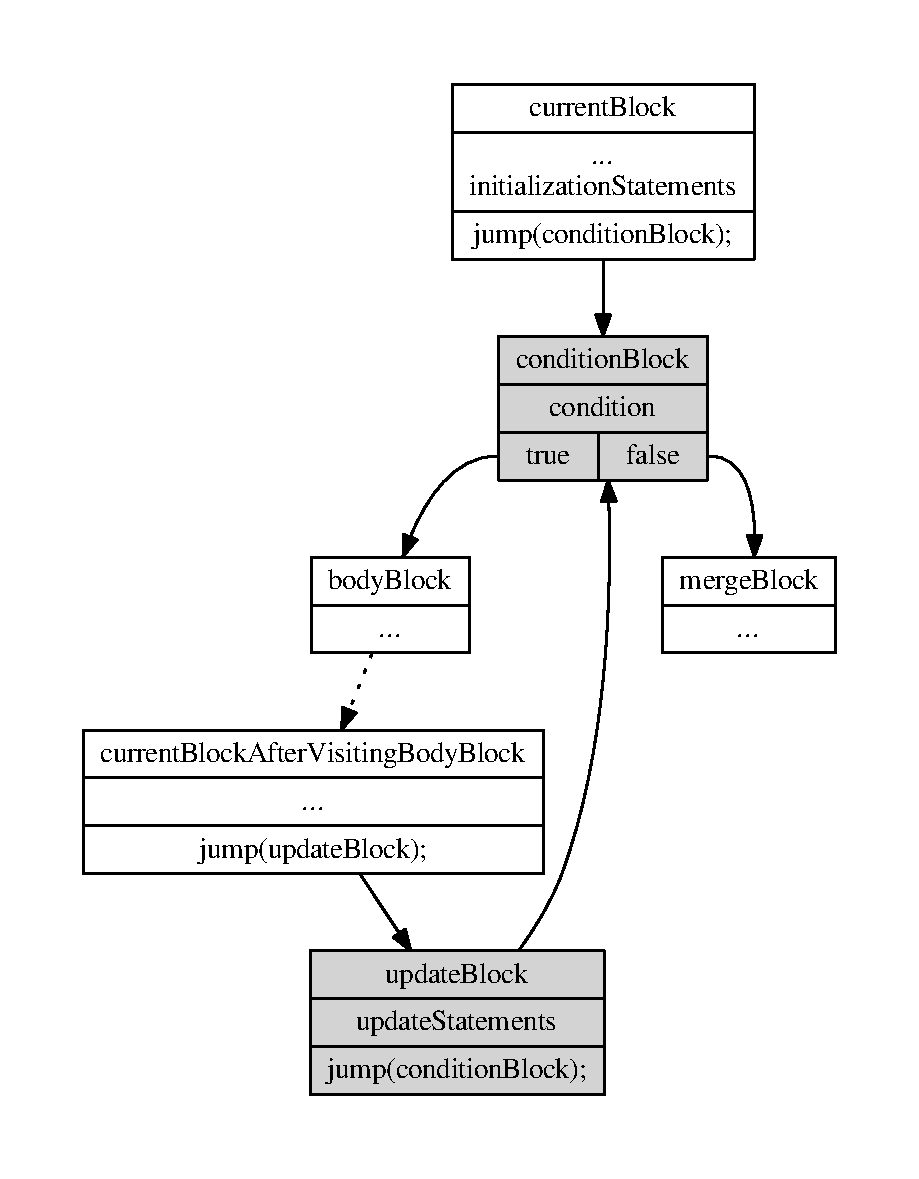
\includegraphics[width=\textwidth]{src/graph/for.pdf}
        \caption{For statement CFG\label{img:for-statement}}
    \end{subfigure}%
    \begin{subfigure}[b]{0.4\textwidth}
        \centering
        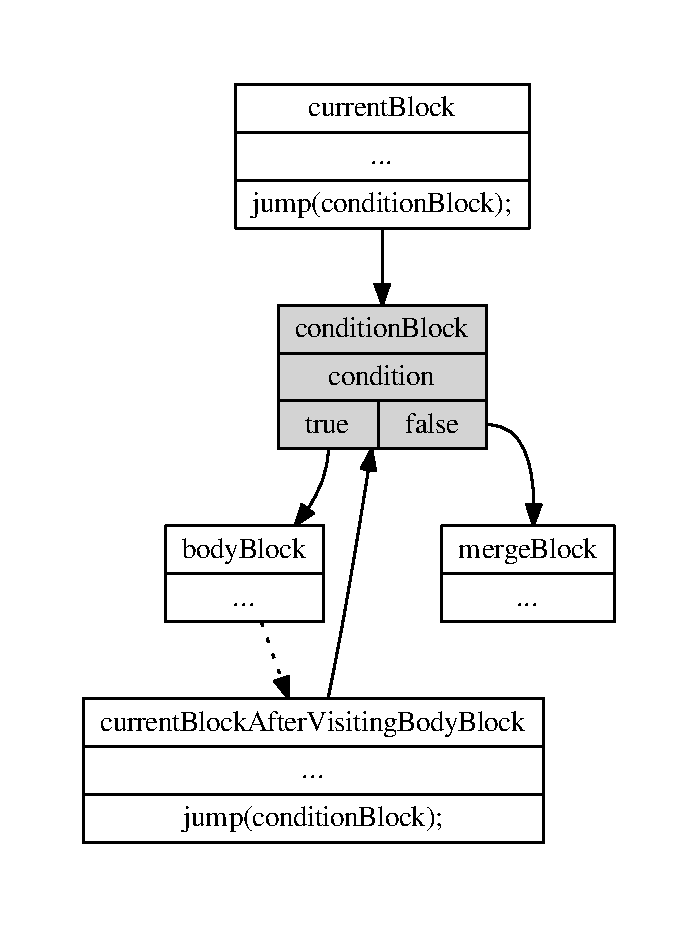
\includegraphics[width=\textwidth]{src/graph/while.pdf}
        \caption{While statement CFG\label{img:while-statement}}
    \end{subfigure}%
    \begin{subfigure}[b]{0.4\textwidth}
        \centering
        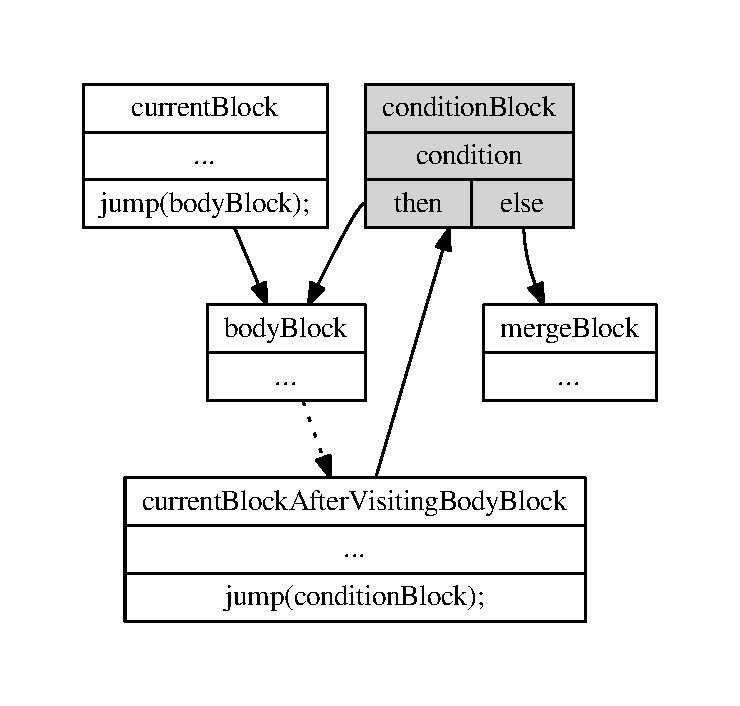
\includegraphics[width=\textwidth]{src/graph/do-while.pdf}
        \caption{Do-while statement CFG\label{img:do-while-statement}}
    \end{subfigure}
    }
    \caption{Loop statements CFGs\label{img:loop-statement}}
\end{figure}

\subsection{Visiting a \code{PsiSwitchStatement}}

After the \textit{Replacing single statements with block statements} pass, the body of a \code{switch} statement
contains only either \code{PsiSwitchLabelStatement}s or \code{PsiBlockStatement}s.

First, a \code{mergeBlock} is generated, the \code{myCurrentBlock} is saved in an \code{oldCurrentBlock} variable and
the \code{previousCurrentBlock} is set to \code{null}. An empty list of \code{Statement}s called \code{statements}
is also initialized. Then each statement in the body of the \code{switch} statement is processed.

If the current statement is an instance of \code{PsiSwitchLabelStatement}, then a\\
\code{NormalStatement} wrapping the \code{PsiSwitchLabelStatement} is added to the \code{statements} list.

If the current statement is an instance of \code{PsiBlockStatement}, then a \code{newBlock} is created and an
\code{UnconditionalJumpStatement} to this \code{newBlock} is added to the \code{statements} list. If the
\code{previousCurrentBlock} is not \code{null} and it is not finished (its last statement is not a
\code{TerminatorStatement}), then an \code{UnconditionalJumpStatement} to the \code{newBlock} is added to the
\code{previousCurrentBlock}. This happens when the control flow falls through the \code{previousCurrentBlock} to
the \code{newBlock}. Then the \code{myCurrentBlock} is set to \code{newBlock} and the visitor visits the current
\code{PsiBlockStatement}. After this, the \code{previousCurrentBlock} is set to the actual \code{myCurrentBlock},
which may be other than before the visitor visits the \code{PsiBlockStatement}.

After processing all the statements in the \code{switch} body, if the \code{previousCurrentBlock} is not \code{null}
and it is not finished, an \code{UnconditionalJumpStatement} to the \code{mergeBlock} is added to the
\code{previousCurrentBlock}. This happens when control flow falls through the last block in the \code{switch} body to
the \code{mergeBlock}.

Then the \code{myCurrentBlock} is restored from \code{oldCurrentBlock} and a \code{SwitchStatement} is added to the
\code{myCurrentBlock}, containing the the \code{PsiExpression} associated with the \code{PsiSwitchStatement} and the
computed \code{statements} list. The \code{myCurrentBlock} is then set to the \code{mergeBlock}.

An example of the generated basic blocks is provided in \labelindexref{Figure}{img:blocks}. Each block is assigned to
a \code{case} inside a \code{switch} statement which replaces the incorporated body of the method. The \code{switch}
statement has the \code{block} field of the \code{frame} object as its expression. The CFG of the method body can be
better visualized in the \labelindexref{Figure}{img:cfg}. There are two basic blocks with \code{id}s equal to \code{6}
and \code{3}, which are unreachable from the first block of the CFG (with \code{id} equal to \code{0}). The red lined
blocks are blocks which should explicitly not be inlined, because they are blocks which appear after a recursive call or
because the number of incoming blocks is not equal to \code{1} (it is \code{0} in this particular case).

\begin{figure}[htb]
    \makebox[\linewidth][c]{%
    \begin{subfigure}[b]{.6\textwidth}
        \centering
        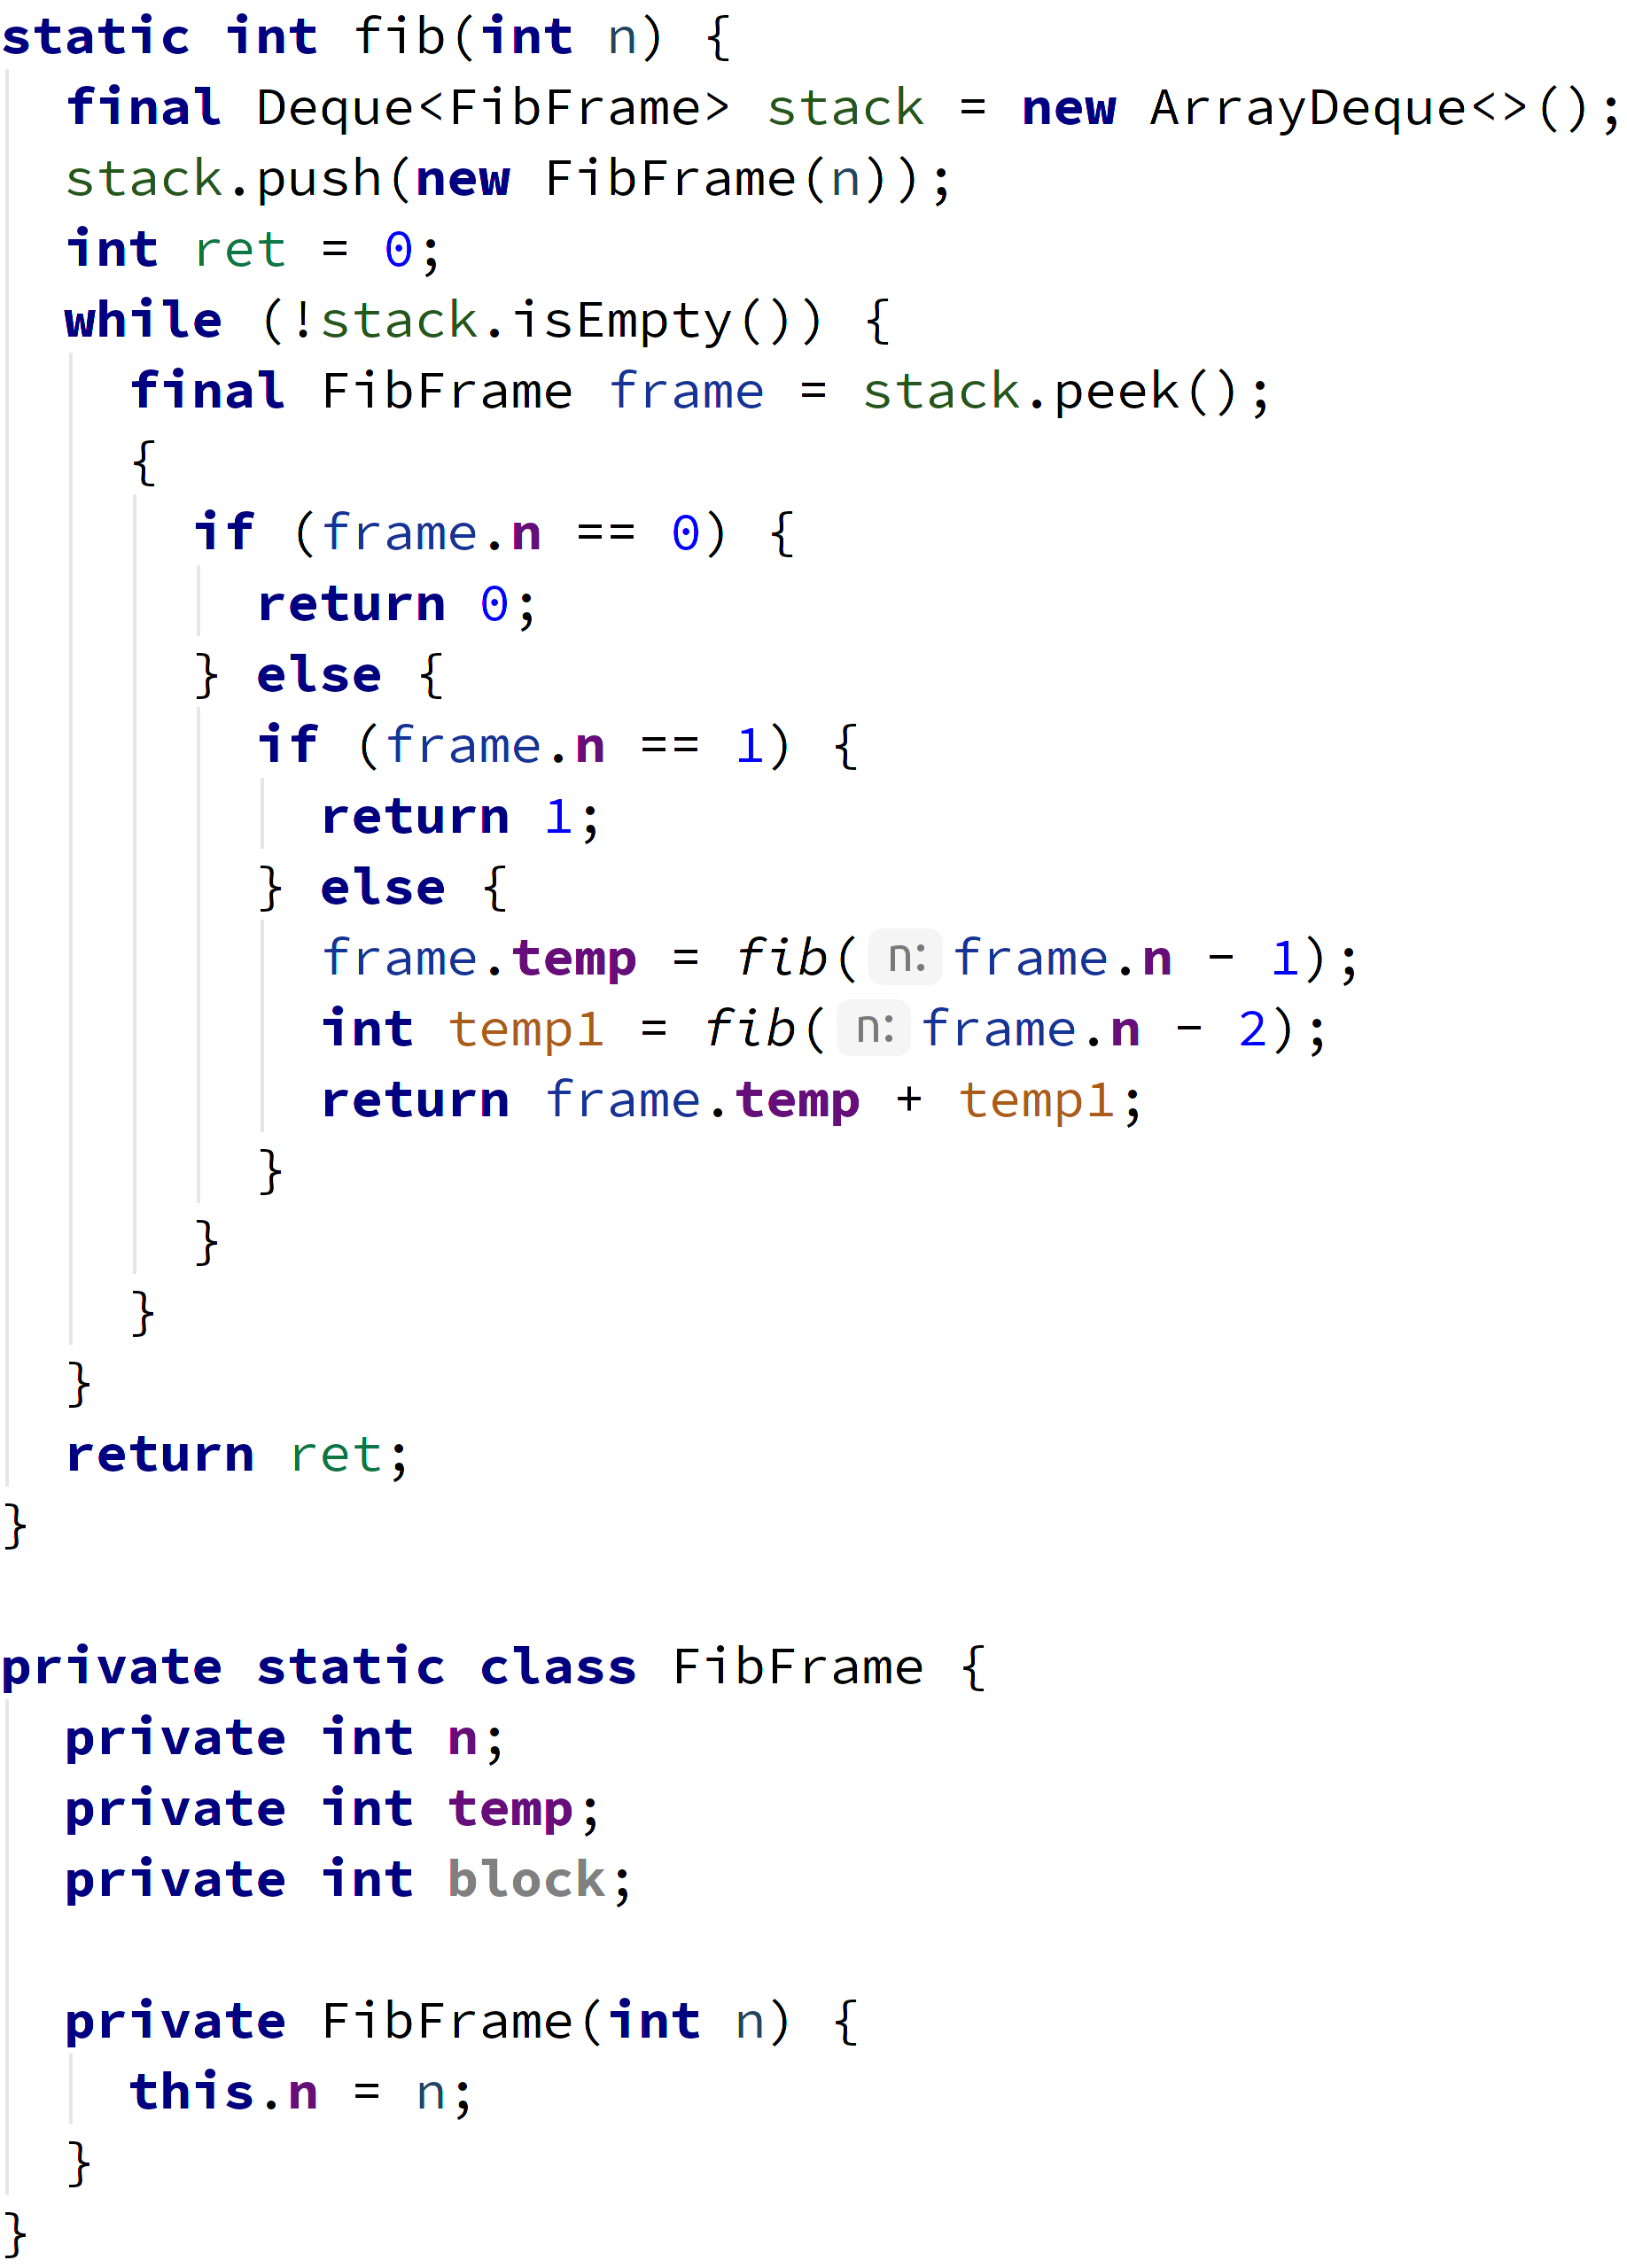
\includegraphics[height=3in]{src/img/cfg-before-white-32.png}
        \caption{Before}
    \end{subfigure}%
    \begin{subfigure}[b]{.6\textwidth}
        \centering
        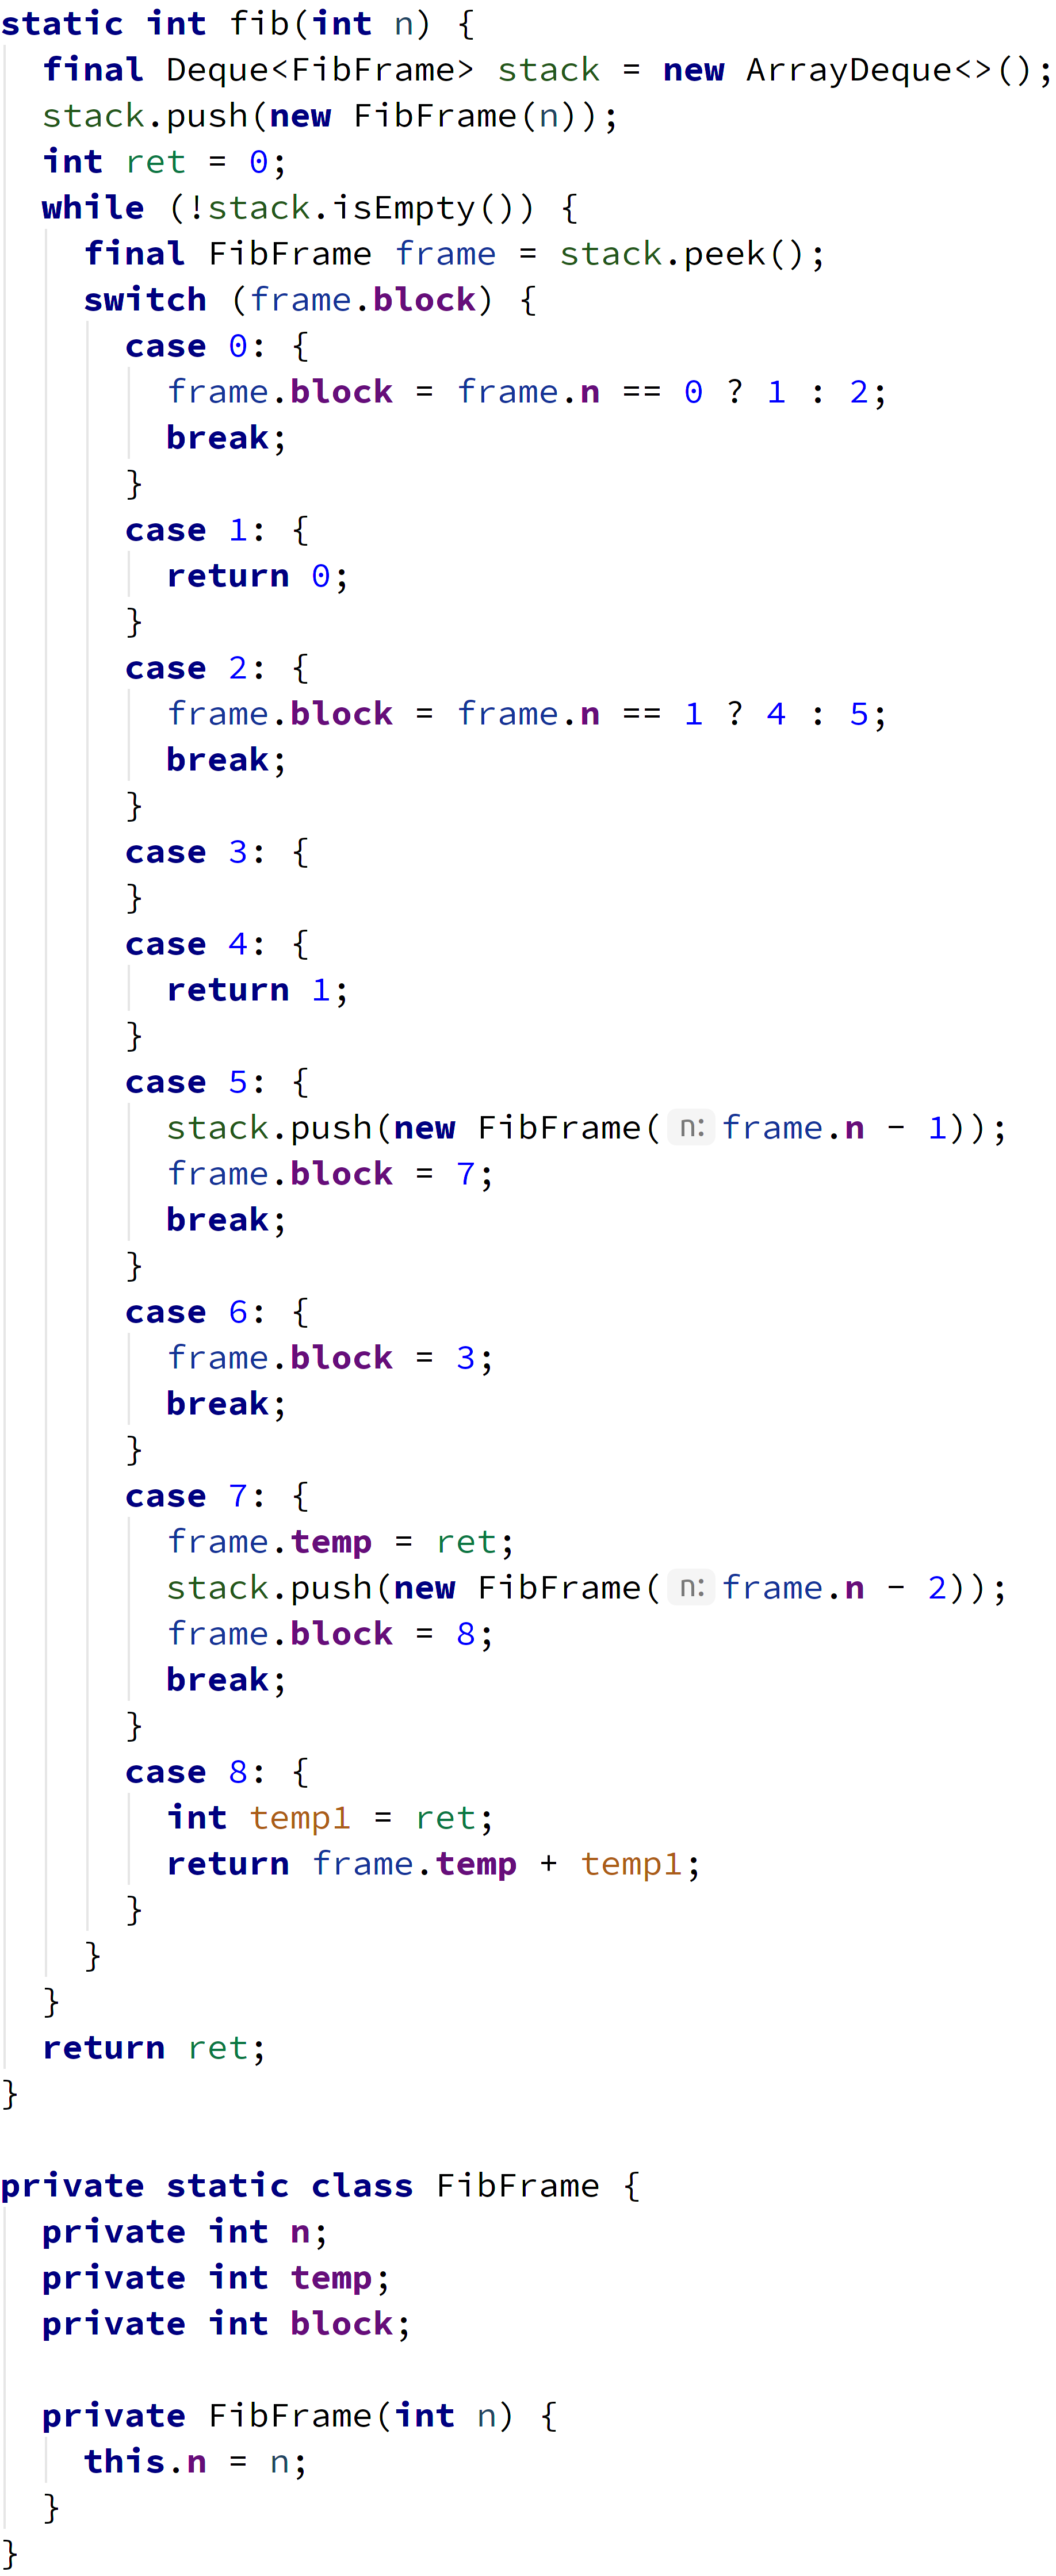
\includegraphics[height=5.25in]{src/img/cfg-after-white-56.png}
        \caption{After}
    \end{subfigure}%
    }\\
    \caption{Generating the control flow graph \label{img:blocks}}
\end{figure}

\begin{figure}[htb]
    \centering
    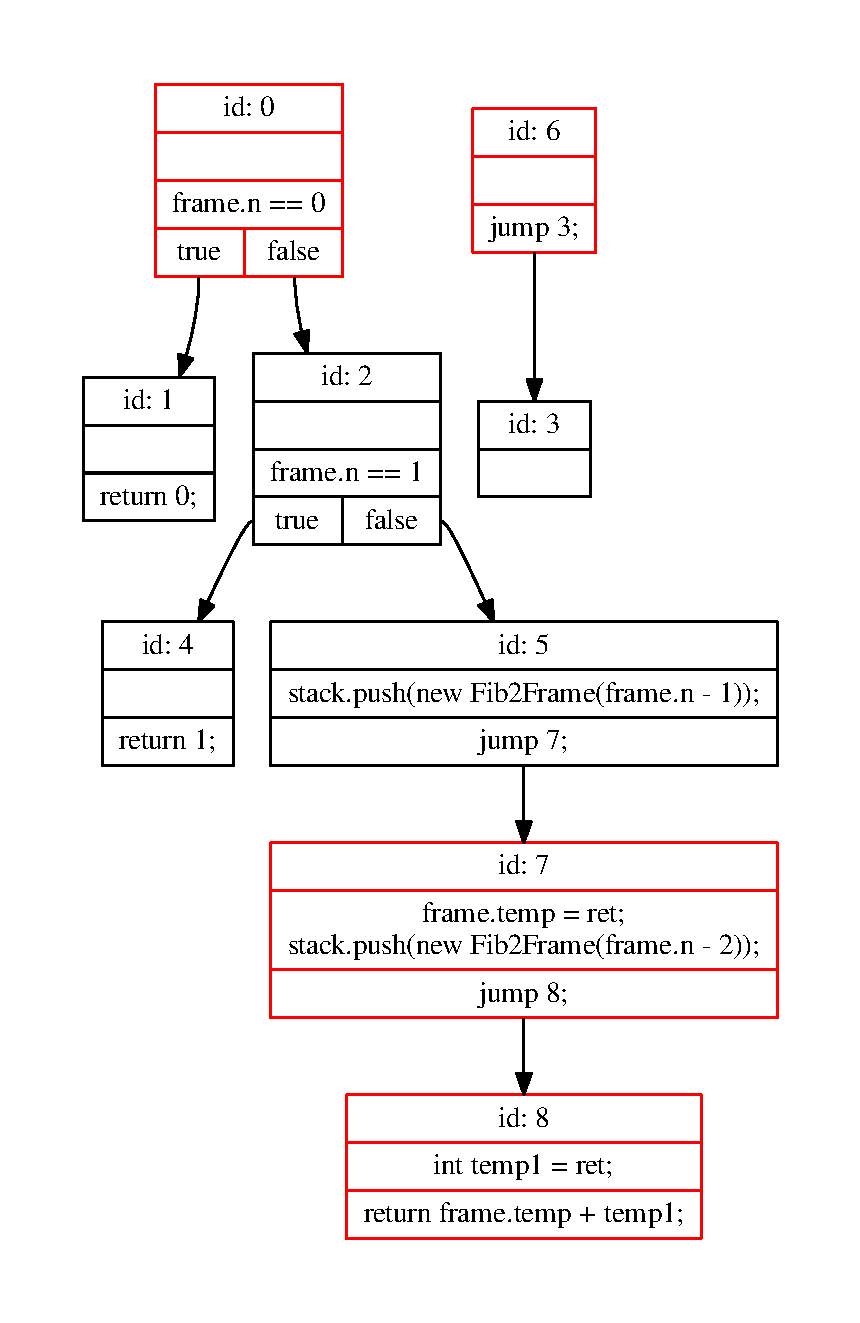
\includegraphics[width=.5\textwidth]{src/graph/cfg.pdf}
    \caption{The CFG\label{img:cfg}}
\end{figure}
